\documentclass[border=2pt]{standalone}
\usepackage{tikz}
\usepackage{amsmath}
\usepackage{mathtools}
\usetikzlibrary{arrows.meta,chains,%
                    decorations.pathreplacing}
\usetikzlibrary{matrix,positioning,arrows.meta,arrows}

\tikzset{
mymat/.style={
  matrix of nodes,
  nodes in empty cells,
  text height=2.5ex,
  text depth=0.75ex,
  text width=3.25ex,
  align=center,
  column sep=-\pgflinewidth
  }
}
\tikzset{
  rows/.style 2 args={
    sub@rows/.style={row ##1 column #2/.style={nodes={rectangle,draw=black}}},
    sub@rows/.list={#1}
  },
  box/.style 2 args={
    sub@box/.style={rows={#1}{##1}},
    sub@box/.list={#2}
  }
}
\begin{document}

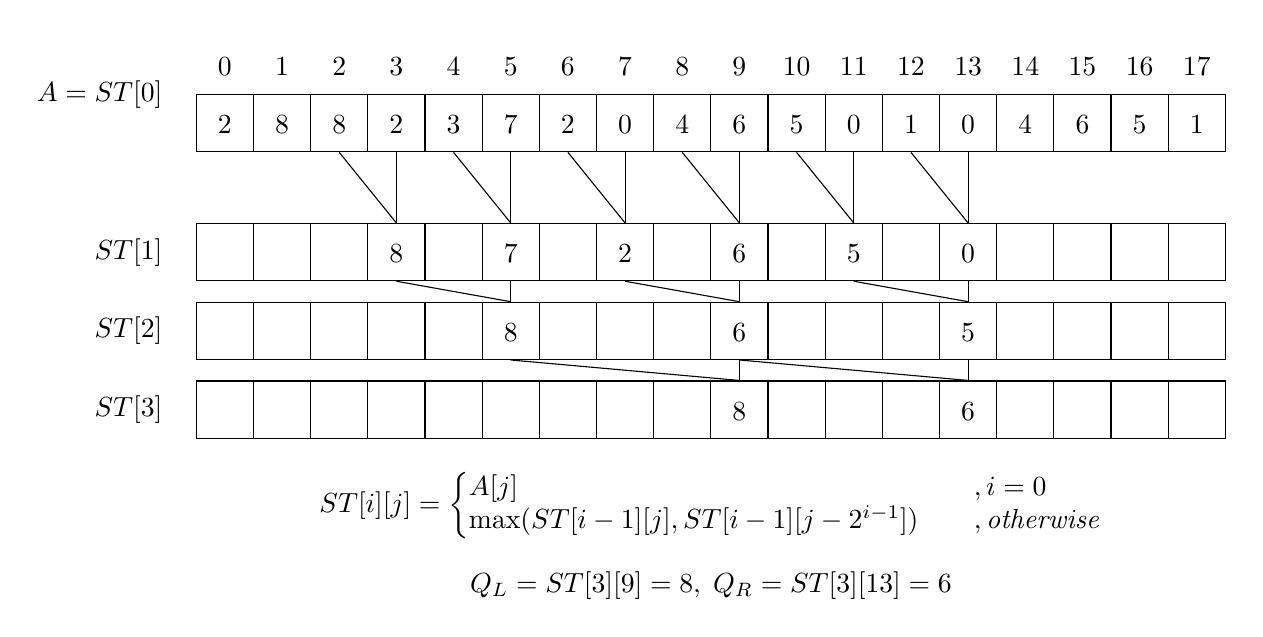
\begin{tikzpicture}[>=latex]


\matrix[mymat,anchor=west,
    box={2}{1, 2, 3, 4, 5, 6, 7, 8, 9, 10, 11, 12, 13, 14, 15, 16, 17, 18}]
at (0,0) 
(mat1)
{ 
  0 & 1 & 2 & 3 & 4 & 5 & 6 & 7 & 8 & 9 & 10 & 11 & 12 & 13 & 14 & 15 & 16 & 17 \\
  2 & 8 & 8 & 2 & 3 & 7 & 2 & 0 & 4 & 6 &  5 &  0 &  1 &  0 &  4 &  6 &  5 &  1 \\};

\matrix[mymat,anchor=west,
    box={1}{1, 2, 3, 4, 5, 6, 7, 8, 9, 10, 11, 12, 13, 14, 15, 16, 17, 18}]
at (0,-2) 
(mat2)
{ 
    &   &   & 8 &   & 7 &   & 2 &   & 6 &    &  5 &    &  0 &    &    &    &     \\};

\matrix[mymat,anchor=west,
    box={1}{1, 2, 3, 4, 5, 6, 7, 8, 9, 10, 11, 12, 13, 14, 15, 16, 17, 18}]
at (0,-3) 
(mat3)
{ 
    &   &   &   &   & 8 &   &   &   & 6 &    &    &    &  5 &    &    &    &     \\};

\matrix[mymat,anchor=west,
    box={1}{1, 2, 3, 4, 5, 6, 7, 8, 9, 10, 11, 12, 13, 14, 15, 16, 17, 18}]
at (0,-4) 
(mat4)
{ 
    &   &   &   &   &   &   &   &   & 8 &    &    &    &  6 &    &    &   &     \\};

\begin{scope}
\draw[]
  (mat3-1-10.south) -- (mat4-1-10.north);
\draw[]
  (mat3-1-6.south) -- (mat4-1-10.north);

\draw[]
  (mat3-1-14.south) -- (mat4-1-14.north);
\draw[]
  (mat3-1-10.south) -- (mat4-1-14.north);

\draw[]
  (mat2-1-14.south) -- (mat3-1-14.north);
\draw[]
  (mat2-1-12.south) -- (mat3-1-14.north);
\draw[]
  (mat2-1-10.south) -- (mat3-1-10.north);
 \draw[]
  (mat2-1-8.south) -- (mat3-1-10.north);
\draw[]
  (mat2-1-6.south) -- (mat3-1-6.north);
 \draw[]
  (mat2-1-4.south) -- (mat3-1-6.north);

\draw[]
  (mat1-2-14.south) -- (mat2-1-14.north);
\draw[]
  (mat1-2-13.south) -- (mat2-1-14.north);
\draw[]
  (mat1-2-12.south) -- (mat2-1-12.north);
\draw[]
  (mat1-2-11.south) -- (mat2-1-12.north);
\draw[]
  (mat1-2-10.south) -- (mat2-1-10.north);
\draw[]
  (mat1-2-9.south) -- (mat2-1-10.north);
\draw[]
  (mat1-2-8.south) -- (mat2-1-8.north);
\draw[]
  (mat1-2-7.south) -- (mat2-1-8.north);
\draw[]
  (mat1-2-6.south) -- (mat2-1-6.north);
\draw[]
  (mat1-2-5.south) -- (mat2-1-6.north);
\draw[]
  (mat1-2-4.south) -- (mat2-1-4.north);
\draw[]
  (mat1-2-3.south) -- (mat2-1-4.north);

\end{scope}

\node[left=5pt of mat1]{ $A = ST[0]$ };

\node[left=5pt of mat2]{ $ST[1]$ };

\node[left=5pt of mat3]{ $ST[2]$ };

\node[left=5pt of mat4]{ $ST[3]$ };

\node[below=5pt of mat4](formula1)
{
  $ST[i][j] = \left\{\begin{matrix*}[l]
    A[j] && , i = 0\\
    \max(ST[i-1][j], ST[i-1][j-2^{i-1}]) && , \textit{otherwise}
  \end{matrix*}\right.$
};

\node[below=5pt of formula1]
{
  $Q_L = ST[3][9] = 8, \; Q_R = ST[3][13] = 6$
};

\end{tikzpicture}

\end{document}